\documentclass{beamer}
\mode<presentation>
\setbeameroption{show notes}

\usepackage{listings} % добавление листингов из исходников
\usepackage{IEEEtrantools} % для создания многострочных математических формул

\usepackage[utf8]{inputenc}
\usepackage[russian]{babel}
\usepackage{pdfpages}
\usepackage{graphicx}
\usepackage{tikz}
\usepackage{xcolor}
\usepackage{multirow}
\usepackage{svg}
\usepackage{textpos}

\usepackage{amsfonts}

% путь к папке с изображениями
\graphicspath{{./img/}}
\setsvg{svgpath = img/} % для svg только

\setbeamertemplate{navigation symbols}{
	\insertframenavigationsymbol
	\raisebox{0.07cm}[0pt][0pt]{
    \insertframenumber/\inserttotalframenumber}
}

\setbeamertemplate{frametitle}[default][center]

% для вывода svg изображения на весь слайд
\newcommand<>{\fullsizegraphic}[1]{
    \vfill
    \begin{textblock*}{0cm}(-1cm,-3.78cm)
    \includesvg[width=\paperwidth]{#1}
    \end{textblock*}
    \vfill
}

\title{The Kernel Recursive Least Squares Algorithm}
\author{Свичкарев Анатолий}

% поля титульного слайда
\institute{Санкт-Петербургский Государственный Политехнический Университет\\
    Петра Великого\\
    \vspace{0.7cm}
    Преподаватель:  к.н. Н.О. Кадырова\\
    \vspace{0.7cm}
}
\date{\today}

\begin{document}

% титульный слайд
\begin{frame}
\titlepage
\end{frame}

% теория
\begin{frame}{Алгоритм}
    \begin{figure}
        \center
        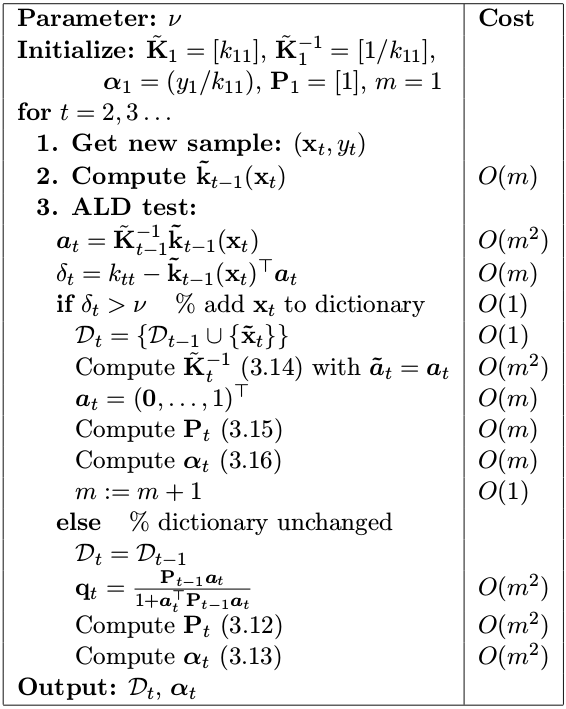
\includegraphics[height=0.8\paperheight]{alg}
    \end{figure}
\end{frame}

\begin{frame}{Root Mean Squared Error}
    Среднеквадратическая ошибка:
    \begin{equation*}
        \textrm{RMSE} = \sqrt{\frac{1}{n} \sum_{i=1}^{n} (f(y_i) - y_i)^2}
    \end{equation*}
    Для Leave-one-out Cross-Validation:
    \begin{equation*}
        \textrm{AverageRMSE} = \frac{1}{k} \sum_{i=1}^{k} \textrm{RMSE}_k
    \end{equation*}
\end{frame}

% тестирование на модели
\begin{frame}{Модельные данные 1}
    \fullsizegraphic{linear}
\end{frame}

\begin{frame}{Модельные данные 2}
    \fullsizegraphic{rbfsin}
\end{frame}

\begin{frame}{Модельные данные 3}
    \fullsizegraphic{rbflinearsin}
\end{frame}

% тестирование на реальных данных
\begin{frame}{Реальные данные}
    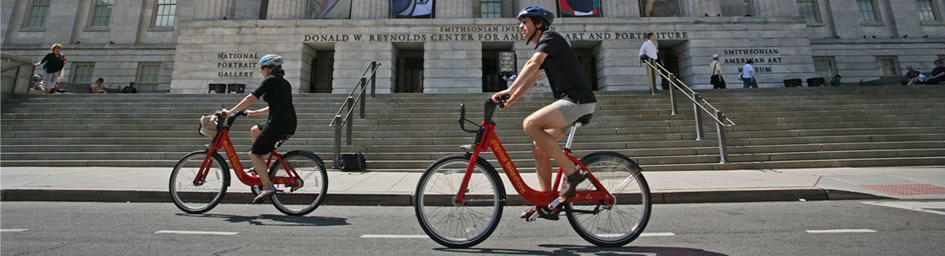
\includegraphics[width=\textwidth]{databike}
    \bigskip

    Ежедневный подсчёт арендованных велосипедов
    за 2011 и 2012 год,
    предоставленные велопрокатной фирмой в Вашингтоне.
\end{frame}

\begin{frame}{Велопрокат в СПб (Реклама)}
    \begin{figure}
        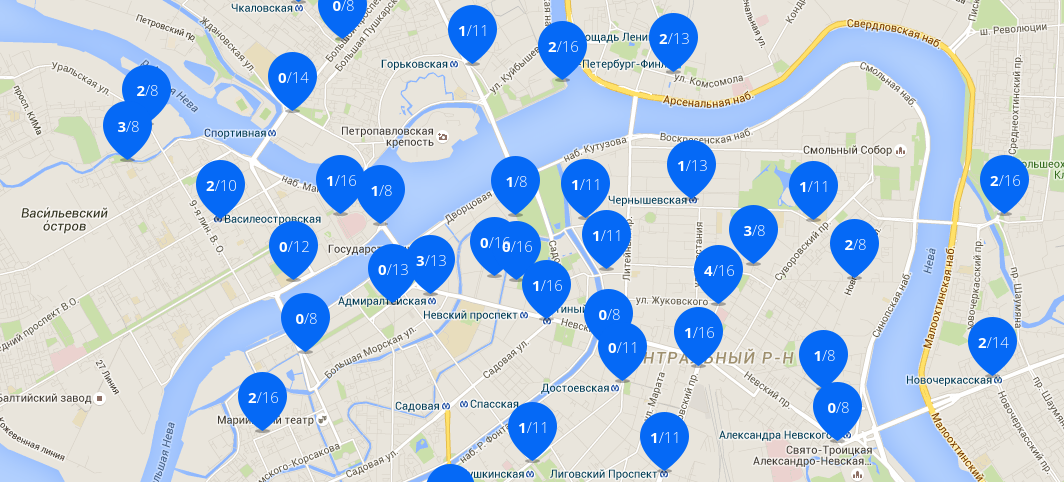
\includegraphics[width=\textwidth]{mapspb}
        \caption{Велостанции и число доступных велоcипедов в СПб.}
    \end{figure}
\end{frame}

\begin{frame}{Реальные данные. Опорные вектора. Попытка 1}
    \fullsizegraphic{sv1}
\end{frame}

\begin{frame}{Реальные данные. Предсказания. Попытка 1}
    \fullsizegraphic{pred1}
\end{frame}

\begin{frame}{Реальные данные. Опорные вектора. Попытка 2}
    \fullsizegraphic{sv2}
\end{frame}

\begin{frame}{Реальные данные. Предсказания. Попытка 2}
    \fullsizegraphic{pred2}
\end{frame}

\end{document}
